% \begin{savequote}[75mm]
% Nulla facilisi. In vel sem. Morbi id urna in diam dignissim feugiat. Proin molestie tortor eu velit. Aliquam erat volutpat. Nullam ultrices, diam tempus vulputate egestas, eros pede varius leo.
% \qauthor{Quoteauthor Lastname}
% \end{savequote}

\chapter{Basic characterizations}
% fig:2p_retino
% fig:rf_examples
% fig:retino_scatter
% fig:rf_aggregate
% fig:vf_coverage

% fig:gratings_examples
% fig:gratings_aggregate
% fig:theta_vs_rf_angle

% Supps:
% rf5_v_rf10
% spherical_correction
% gratings_fitting
% vf_targeting

\newthought{Rats rely on vision} for a many natural behaviors, such as a hunting\cite{REFREF}, jumping and depth perception\cite{REFREF}, and spatial navigation\cite{REFREF}. Over the past few years, a subset of contiguous areas spanning the lateral edge of rat cortex have garnered significant attention due to possible similarities with the primate ventral visual stream. Several studies \cite{Vermaercke2014, Tafazoli2017, Vinken2016NeuralCortex} have investigated these visual areas --- V1, LM, LI, and LL --- specifically in the context of visual object representations in order to test the extent to which single neuron characteristics of primate IT, the highest level of the primate ventral stream, might also be found in the lateral most areas in the rat. 

% Name some known examples for how mice and primates are different.
However, monkeys and rodents, differ in dramatic ways --- on one hand, similarities in how their visual systems solve a given problem are incredibly exciting, as they point to general principles conserved across species. On the other hand, each solution is likely to be influenced by differences in the natural visual statistics by which their visual systems have been shaped. For example, in primates and cats, cells with similar orientation preferences are organized in columnar structures in V1\cite{Blasdel1986}. In contrast, as shown by one of the first two-photon imaging studies of rat V1, and many mouse studies thereafter, rodents have a salt-and-pepper-like organization of orientation preference that does not appear to have an obvious global structure\cite{Ohki2005}). 

Over the past decade, mice have become increasingly popular for studying visual circuits. This is arguably due to the immensely powerful genetic tools combined with chronic, large-scale population recordings, much of which are prohibitively challenging to use in monkeys. In contrast, although rats have long been studied for visually-guided behaviors, large-scale cellular resolution access to their visual cortex has proved to be far more challenging. Our broad-level goal is to bridge the gap between neural circuit access and rich behavioral capacities in the rat. Rats lack a basic characterization of any visual area beyond V1. Such a systematic study provides valuable points of comparison not just with primates, but with other animal models, including mice. 

% ---------------------------------------------------------------
% Experiment design
% ---------------------------------------------------------------
% Broad overview of experiment design -- all the stimuli.
Two overarching goals shaped our experimental design (Figure\ref{fig:experiment_design}). First, we hoped to contribute an immensely powerful method to the existing body of literature on visual object recognition in rats. Several studies have characterized single-unit response properties of lateral extrastriate areas in rats that may be similar to those found in the primate ventral stream\cite{Tafazoli2017, Vermaercke2014, VinkenX, Vermaerke2015}. As such, we know relatively more about single-unit response properties in these lateral areas than in any other extrastriate area of the rat. However, most previous rat studies specifically characterized single-unit responses to object stimuli --- much less is known about more basic response properties of these visual areas. As a parallel goal, we sought to provide a first comprehensive survey of basic, visual response properties across these different cortical areas in the rat using optical imaging. 

% Figure:  Experimental design.
\begin{figure}
    \includegraphics[width=\textwidth]{figures/chapter_3/fig_3-1_experiment_design/fig_3-1_experiment_design.pdf}
    \vspace{.1in}
    \caption[Experiment design]{Experiment design for characterizing visual responses in rat lateral cortex. 
    \textbf{A.} Schematic of the battery of visual stimuli used to characterize rat visual cortex. 
    \textbf{B.} Illustration of how an imaging session proceeded.
    \label{fig:experiment_design}}
\end{figure}

We focused on the first three of four visual areas targeted by previous electrophysiology studies of object recognition properties of rat visual cortex. These areas, V1, LM, and LI, were the most reliably detected with our combined method of viral expression and wide-field mapping, as described in Chapter 2 (given the somewhat inconsistent nature of viral GCaMP expression in terms of even coverage, area LL was not easy to identify with confidence. See the Discussion below). Using a large battery of visual stimuli (Figure\ref{fig:experiment_Design}), we characterized basic visual response properties of these three areas for the first time with cellular resolution imaging. In the same sessions, we also tested a subset of the complex visual object stimuli used to test the perceptual behavior of rats (behavior described in Chapter 1, neural characterizations described in Chapter 4). Given their potential as areas important for visual object recognition behavior, areas V1, LM, and LI  represent an exciting starting point for combining the powerful tools common in traditional genetic models like mice with the kinds of complex behaviors associated with primates.  

\section{Identification of two-photon imaging sites}
The mirror reflections of the retinotopic gradient in our wide-field maps identified macro-level areal borders. We used these maps to determine which visual areas to target for two-photon imaging sessions. In order to register the two-photon maps to the wide-field maps, we acquired an anatomical volume at the start of each session. This was a surface-level z-stack that captured fiduciary markers in both channels: while the green channel was always used for functional runs (GCaMP), we used the red channel to acquire images of blood vessels filled with a temporary fluorescent dye that was injected at the start of each session (see Methods). Acquiring an anatomical volume also helped for identifying and returning to the same FOV across days. 

Each rat underwent a localizer run prior to any functional sessions. Localizer runs were conducted on a day prior to full functional sessions. These sessions identified which parts of the visual field corresponded to a given imaging site, targeted based on the surface-level vasculature and wide-field areal mapping (see Chapter 2, Figure\ref{fig:retino_mapping}). Two-photon vasculature images were matched offline to the high-resolution images we took of the brain surface in each wide-field mapping session. Once a candidate FOV was found to contain visually responsive cells, and the visual area assignment was validated, it was acceptable for full functional runs, which were the full battery of stimuli used to characterize the FOV (Figure\ref{fig:experiment_design}). Localizer runs were always run again during functional sessions.

We used two types of mapping protocols that targeted different scales of retinotopic organization. The first captured broad retinotopic preferences across the field-of-view using the same cycling bar stimulus used to identify area borders in wide-field maps (see Chapter 2, \ref{fig:retino_mapping}). The second provided a more fine-scaled characterization of individual receptive fields for each neuron in the selected FOV:  we used a time-consuming, albeit highly reliable, approach in which small portions of the visual field were systematically stimulated in a tiled manner to estimate the receptive field positions and extents of all cells. In addition, since only a subset of the experiments used full-field stimuli, it was important to accurately identify the region of visual space to which most cells in a given FOV were responsive and target the stimulus presentation there. 

Once a given FOV was identified as visually responsive, and the receptive field locations of the whole population could be identified, functional runs were conducted on subsequent days. We selected a battery of stimuli to provide a foundation for basic visual response properties in the lateral extrastriate areas of the rat. The final stimulus sets included drifting gratings of multiple orientations, spatial frequencies, and speeds, and a subset of the complex object stimuli used to test rats' perceptual behavior (as described in Chapter 1).

% ---------------------------------------------------------------
% 2p retinotopy
% ---------------------------------------------------------------
% fig:2p_retino (2p setup, coregistration, gradient, cortical mag)
% fig:rf_examples (fine-scaled RF measurements)
% fig:retino_scatter 
% fig:rf_aggregate
% fig:vf_coverage
% ---------------------------------------------------------------

\section{Fine-scale retinotopic organization in rat lateral cortex}
While previous studies have relied on coarse retinotopy to identify the areas in which they were recording, the fine-scale retinotopic organization of cell bodies in any extrastriate area remains unknown. Using the same phase-encoding Fourier paradigm we used to measure retinotopic gradients in wide-field maps, we characterized retinotopic preferences across a given two-photon field-of-view (Figure\ref{fig:2p_retino}A). This method also allowed us to quickly identify and validate that the retinotopic gradient direction measured at the macro scale was aligned with the gradient measured in the two-photon FOV. Two-photon FOVs were registered to wide-field vasculature maps offline by selecting matching points between the two views based on uniquely identifiable blood vessels present in both images. We then used these points to identify a transformation matrix to map one view onto the other (Figure\ref{fig:2p_retino}B, and see Methods). Sweeps of the cycling bar produced robust responses in individual cells throughout the FOV (Figure\ref{fig:2p_retino}D). We observed retinotopic gradients across visual axes of elevation (ventral-dorsal) and azimuth (nasal-temporal) for FOVs imaged in V1, LM and LI (Figure\ref{fig:2p_retino}E). 

% fig:2p_retino 
\begin{figure}
    \includegraphics[width=\textwidth]{figures/chapter_3/fig_3-1_2p_retino/fig_3-1_2p_retino.pdf}
    \vspace{.1in}
    \caption[Identification of areas with two-photon imaging]{Coregistration and area identification for two-photon imaging. \textbf{A.} Schematic of imaging experiments in awake, head-fixed rats. 
    \textbf{B.} \textit{Left}: Wide-field image of the surface vasculature in the cranial window of an example rat. The overlay (blue) shows the co-registered anatomical image of the surface vasculature acquired by two-photon imaging. Scale bar, 1mm. 
    \textbf{C.} Example two-photon imaging field-of-view using the standard, large-FOV mode. The FOV is scaled for visualization purposes based its measured pixel size. Scale bar, $100um$. 
    \textbf{D.} Example z-scored timecourses for three cycles of the moving bar stimulus for all identified cells in an imaging site. Condition shown was a white bar (5 degrees of visual angle) moving in the nasal-to-temporal direction across the screen at 0.24Hz. Traces are colored and sorted by each cell's phase at the stimulation frequency (colormap as in \textbf{E}). Dotted lines denote the start of each cycle. 
    \textbf{E.} Pseudo-colored image of retinotopic azimuth (left) and elevation (right) preference obtained by two-photon imaging with the cycling bar stimulus, \textif{i.e.}, the same phase-encoded mapping paradigm used for wide-field mapping. Colors within cell body masks indicate preferred retinotopic locations. Background pixels contain a smoothed estimate of neuropil retinotopic preferences. 
    \textbf{F.} Cortical magnification for each imaging site recorded in areas V1, LM and LI (*: p<0.05, **: p<0.01, Mann-Whitney U-test, REFREF corrected for multiple comparisons). 
    \textbf{G.} Ratio of cortical magnification along elevation to azimuth for each imaging site. Conventions as in \testbf{F}.   
    \label{fig:2p_retino}}
\end{figure}

% ---------------------------------------------------------------
% Cortical magnification
% ---------------------------------------------------------------
\subsection{Cortical magnification is asymmetric}
The particular region and extent of visual space that a patch of cortex represents has important implications for its function. For example, in primates, most areas of the ventral stream over-represent the central visual field, enhancing the processing of features near the fovea\cite{REFREF, Gattass2005CorticalDynamics}. Although mice and rats do not have foveal vision, several groups have shown biases of visual field coverage across visual cortex in mice\cite{Garrett2014, Marshel2011, REFREF}. To quantify how much surface area is devoted to a given unit of visual space in rat extrastriate cortex, we measured cortical magnification in areas V1, LM and LI. Overall, we found that cortical magnification decreased from V1 to LM to LI, consistent with the expectation that larger areas have more cortical real estate for representing a given part of visual space (Figure\ref{fig:2p_retino}F). 

Cortical magnification is not necessarily isotropic, that is, equal along vertical (azimuth) and horizontal (elevation) axes of the visual field. We found an asymmetric expansion along the vertical dimension of visual space in rat V1, as well as in areas LM and LI (Figure\ref{fig:2p_retino}G). This asymmetry is consistent with findings in mouse V1, in which several studies have reported an expanded representation along the vertical dimension of visual space\cite{Garrett2014, Liang2018, Bonin2011}.  

% ---------------------------------------------------------------
% RFs for better measurements (rfs5 vs rfs10)
% ---------------------------------------------------------------
\subsection{Retintopy is disorganized at fine scales}
Interestingly, we observed slight deviations when comparing our smoothed gradient maps to estimated retinotopic preferences of cell bodies (see Figure\ref{fig:2p_retino}E). Previous studies in mouse visual areas indicate the presence of a fine-scale retinotopic scatter from retinal ganglion cell (RGC) inputs, through the lateral geniculate nucleus (LGN), and into V1 and LM\cite{Liang2018, Andermann2011, Marques2018}. However, it remains unknown whether this scatter is present in other extrastriate areas of rodent cortex, and whether this is functionally advantageous in any way or only a byproduct of biological noise. In order to more finely characterize retinotopic preferences of individual cells, we quantified receptive field (RF) properties by stimulating tiled locations across the visual field (Figure\ref{fig:rf_examples}). 

% fig:rf_examples
\begin{figure}[t!]
    \includegraphics[width=\textwidth]{figures/chapter_3/fig_3-2_rf_examples/fig_3-2_rf_examples.pdf}
    \vspace{.1in}
    \caption[Receptive field mapping]{Mapping receptive fields of single neurons. \textbf{A.} REFREF.
    \label{fig:rf_examples}}
\end{figure}

We used tile sizes of 5 or 10 degrees of visual angle to account for the possibility that cells with larger receptive fields may not be effectively stimulated by small stimuli, and vice versa, that cells with small receptive fields or sensitivity to surround suppression may be under-stimulated by large stimuli. Consistent with previous studies that mapped receptive fields in mice\cite{DeVries2019}), the larger, 10 degree tile size produced more and stronger responses for cells in extrastriate area LI, while the 5 degree tile size worked well for areas V1 and LM. To confirm that the stimulus size did not dramatically affect any of our receptive field measurements, we directly compared the receptive fields of cells in which we obtained fits using both the small and large stimulus sizes (REFREF Figure\ref{fig:suppfig}). Overall, we found that V1 cells had slightly underestimated receptive field sizes when using the larger stimulus size. Importantly, for the goal of obtaining precise retinotopic position estimates for each cell, defined as the center of the fit receptive field, receptive field position meaured with small and large stimuli were tightly correlated, for both azimuth and elevation positions (Supplemental Figure\ref{suppfig:rf5_rf10} REFREF). We did not observe systematic biases in any of the other receptive field metrics, and thus selected whichever of the two stimulus sizes produced the most well-fit receptive fields on average for LM (smaller, 5-degree tile size) and LI (larger, 10-degree tile size). 

% ---------------------------------------------------------------
% \subsection{Retinotopic scatter is asymmetric}
% Average cortical scatter
% ---------------------------------------------------------------
To quantify scatter, we compared measured receptive field positions to predicted positions. Specifically, for a given population of cells recorded at an imaging site, we calculated the global retinotopic gradient using smoothed estimates of neuropil preferences across the FOV (Figure\ref{fig:retino_scatter}A). Since the vertical and horizontal axes of the visual field representation is not necessarily aligned to anterior-posterior or medial-lateral axes of the cortical surface, we computed a simple transformation that identified the directions of maximal change along each direction based on the smoothed neuropil retinotopic map. Specifically, to compute the spatial axis corresponding to the global retinotopic gradient for each axis, we used the average gradient vector across the FOV. The smoothed retinotopic map was then 
projected along this mean gradient vector, and the predicted location of each pixel was defined as its projected location along this new spatial axis (see Methods).  

After making this correction, we found that most cell bodies exhibited a coarse-scale retinotopic organization (Figure\ref{fig:retino_scatter}B), Pearson's correlation coefficient, V1: r=REFREF, p<0.01; LM: r=REFREF, p<0.01; LI: r=REFREF, p<0.01). However, at the level of neighboring cells, retinotopic preferences were disordered and deviated from the expected preferences based on relative cortical location. To ensure the observed scatter was not simply measurement noise, we identified true deviants by estimated 95\% confidence intervals for all measured receptive field positions. Specifically, for each cell, we determined whether the 95\% confidence interval estimated for its receptive field position along the vertical or horizontal axes overlapped with the 95\% confidence interval estimated for the linear fit defining its predicted receptive field locations based on cortical position.  

\begin{figure}[t!]
    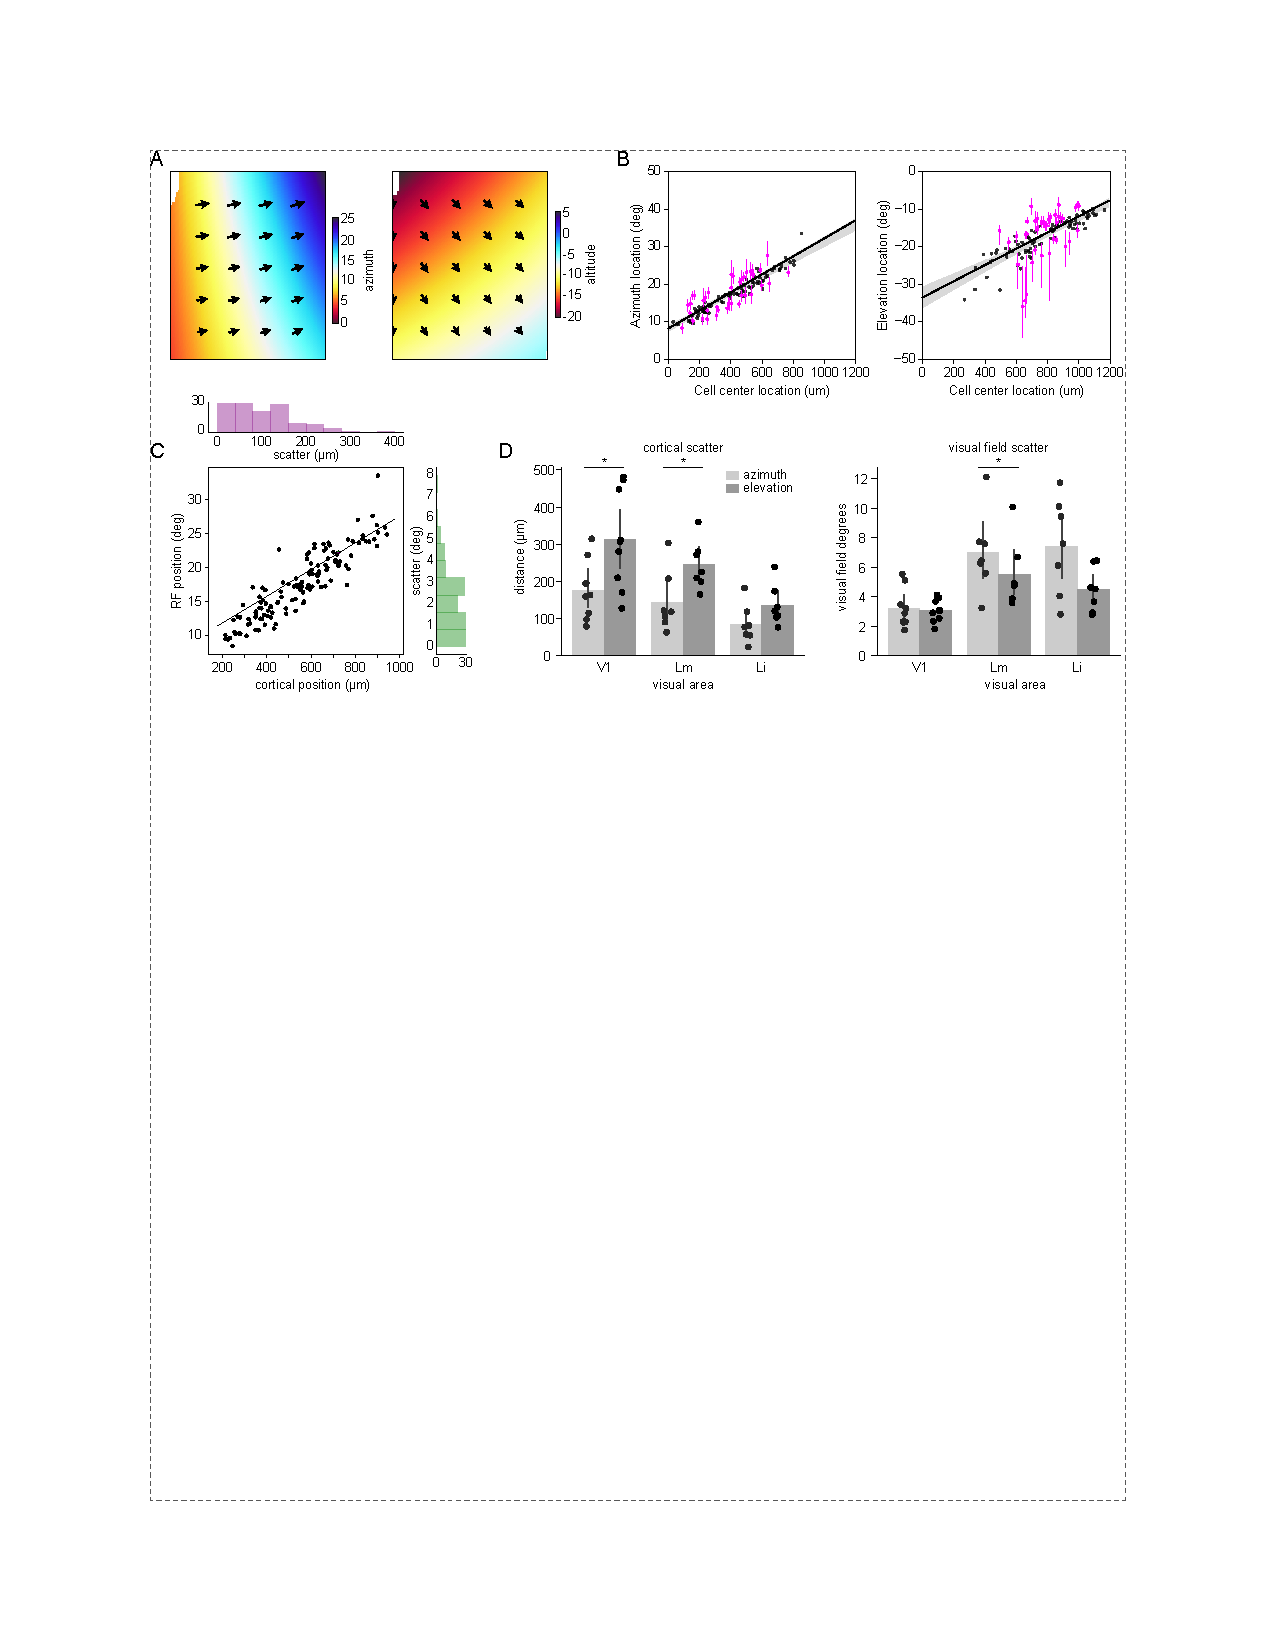
\includegraphics[width=\textwidth]{figures/chapter_3/fig_3-3_retino_scatter/fig_3-3_retino_scatter.pdf}
    \vspace{.1in}
    \caption[Fine-scale retinotopic scatter]{Fine-scale retinotopic scatter in lateral extrastriate cortex. 
    \textbf{A.} Smoothed estimates of neuropil retinotopic preferences for an example V1 FOV for azimuth (left) and elevation (right). Colormap shows visual field position in degrees of visual angle.
    \textbf{B.} Each cell's retinotopic preference versus cortical location along azimuth (left) and elevation (right) axes of retinotopic progression for the example field of view shown in \testbf{A}. Black line: linear fit to retinotopic gradient. Shaded bands, 95\% CI. Black dots: individual cells in the field of view for which reliable receptive field estimates were made (see Methods). Magenta dots: True deviants that significantly deviated from predictions. Magenta lines, 95\% CI. 
    \testbf{C.} Illustration of scatter in cortical position (purple) and scatter in visual field position (green) based on predicted retinotopic preferences based on cortical position. Line, linear fit of the predicted retinotopic gradient, based on the projection of the neuropil map onto the mean gradient vector (as shown in \textbf{A}). Dots, measured receptive field position and cortical position for each cell in an example FOV. Green vertical line indicates deviation in preference from the mean retinotopic gradient ("visual field scatter" in degrees of visual angle scatter). Purple horizontal line indicates the distance of a cell from its expected cortical location in the absence of scatter ("cortical distance scatter" in $um$). 
    \textbf{D.} Average amount of scatter in cortical distance (left) and visual field position (right) for each imaging site recordedin areas V1, LM, and LI. Each dot represents scatter along azimuth (light gray) or elevation (dark gray) for a given FOV.
    \label{fig:retino_scatter}}
\end{figure}

% Overall scatter & asymmetric scatter in X, Y
To quantify the scale of scatter, that is, the extent to which scatter in the receptive field position corresponds to or is offset by scatter in a cell's cortical position, we measured deviations along cortical distance and visual field position for each cell (Figure\ref{fig:retino_scatter}C). Overall, average scatter in cortical space decreased from V1 to LM to LI (Figure\ref{fig:retino_scatter}D, V1: $\sim$239.09+/-REFREF$um$, Lm: $\sim$163.48+/-REFREF$um$, Li: $\sim$127.17+/-REFREF$um$), corresponding to average retinotopic displacements that increased from V1 to LM to LI (V1: $\sim$2.9; LM: $\sim$5.3; LI: $\sim$6.5 degrees of visual angle). This relative pattern is consistent with the relatively smaller cortical size of areas LM and LI relative to V1 (that is, larger area, more room for error).  

Notably, the observed retinotopic scatter was asymmetric between vertical and horizontal dimensions:  deviations from predicted cortical locations were ~2 fold larger along elevation than azimuth (V1: REFREF in azimuth, REFREF in elevation; Lm: REFREF in azimuth, REFREF in elevation; Li: REFREF in azimuth, REFREF in elevation). In V1, this asymmetric scatter in cortical position was roughly proportional to cortical magnification --- that is, for a given unit of visual field space, we observed $\sim$2-fold expansion in cortical space  for elevation, relative to azimuth, and we see a proportional amount of scatter. In LM and LI, however, we observed less scatter in predicted receptive field positions along the elevation axis than would be expected from the measured cortical scatter if scatter was proportional to the cortical magnification of elevation over azimuth.


% ---------------------------------------------------------------
% RF properties
% ---------------------------------------------------------------
% RFs are anisotropic, elongated along azimuth
% -better resolution in elevation? -- horizontally oblong
Given the observed asymmetry in cortical magnification along azimuth and elevation (see Figure\ref{fig:retino_scatter}), we asked whether this asymmetry was also present at the level of individual receptive field shapes. A hallmark of hierarchically-organized visual areas, based on the primate ventral stream, is a gradual increase in average receptive field size\cite{RustREFREF, Vermaerke2014, Siegle2019AAreas, Tafazoli2017}. We quantified overall receptive field size as the average widths along the horizontal and vertical axes (Figure\ref{fig:rf_aggregate}A). Consistent with previous electrophysiology measures in rats\cite{Vermaercke2014, Tafazoli2017}, we found that average receptive field size increased from V1 to LM to LI (V1: median 8.8+/-REFREF, LM: 10.5+/-REFREF degrees, LI: 13.1+/-REFREF degrees of visual angle, p<0.01, Mann-Whitney U-test, p<0.01, fdr-bh corrected for multiple comparisons REFREF). This was true regardless of whether comparisons were restricted only to cells fit using either the small or large stimulus size for all visual areas (Figure\ref{fig:Supp} REFREF).  

% Interestingly, the amount of scatter in the predicted receptive field locations corresponded to roughly half or less than the average receptive field size of each visual area (REFREF, V1: ~$9.49+/-REFREF$, Lm: ~$10.61+/-REFREF$, LI: ~$13.25+/-REFREF$ degrees of visual angle). However, at the level of individual cells, we observed no correlation between receptive field size and retinotopic scatter (Supp Figure REFREF), stats, Pearson’s correlation, V1: REFREF, p=REFREF, Lm: REFREF, p=REFREF, Li: REFREF, p=REFREF).

\begin{figure}[t!]
    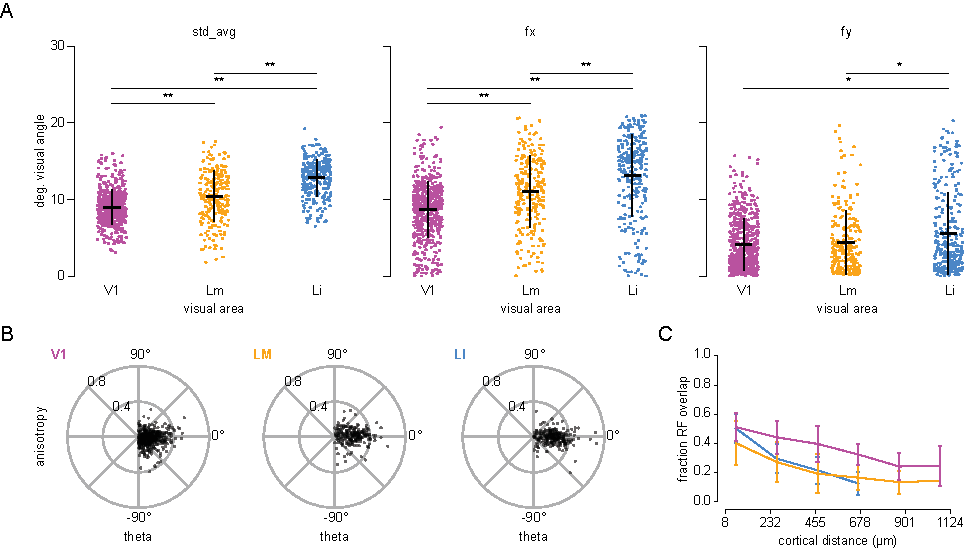
\includegraphics[width=\textwidth]{figures/chapter_3/fig_3-4_rf_aggregate/fig_3-4_rf_aggregate.pdf}
    \vspace{.1in}
    \caption[Receptive field properties]{Receptive field properties across lateral extrastriate cortex. 
    \textbf{A.} \textit{Left}: Average size, measured as half-width at half-max (HWHM) of a double Guassian fit. Also shown is the projection of the major axis of each ellipse onto the horizontal (\textit{middle}) or vertical (\textif{right}) axes of visual space for each cell. Each dot represents one cell. Horizontal and vertical bars, mean and SD across cells. 
    \textbf{B.} Anisotropy, measured as the ratio of major to minor axes of the fit ellipse, as a function of receptive field angle. Each dot is a cell. Anistropy ranges from 0 to 1, where 0 represents perfectly isotropic receptive fields (a circle), and 1 represents an extremely linear receptive field. Receptive field angles of 0 represent orientations parallel to the horizontal axis, and 90 degrees represents orientation parallel to the vertical axis.
    \textbf{C.} Receptive field overlap as a function of cortical distance. For each pair of cells, overlap is measured as the intersection of their receptive fields divided by their union. Error bars, SD.  
    \label{fig:rf_examples}}
\end{figure}

Interestingly, when we split receptive field size according to the extent of vertical or horizontal space covered, we found that the horizontal dimension was consistently larger, suggesting that most receptive fields were anisotropic (Figure\ref{fig:rf_aggregate}A). For each cell, we calculated the degree of anisotropy by taking the ratio of the major and minor axes of the fit ellipses. Most receptive fields exhibited some degree of anisotropy, with receptive field angles biased toward 0 degrees, elongated along their azimuthal dimension (Figure\ref{fig:rf_aggregate}B). 
% However, we did not observe strong relationships between anisotropy and retinotopic scatter (REFREF, Supplemental 3.3) nor between angular bias in anisotropy (horizontally or vertically anisotropic, see Methods) and retinotopic position (REFREF, Supplemental 3.4). 
% -Sit & Goard, bias for cells representing LOWER visual field, stronger coherent motion response -- spatial asymmetry in motion representation/sensitivity

% Spherical correction check:
% ---------------------------------------------------------------
To confirm that the observed receptive field anisotropy was not simply due to variable screen distance, we calculated the same metrics with a spherical correction. Typically, in visual field mapping studies, the screen is close enough to the animal's eye that significant warping can occur at the edges of the visual field, relative to the portions directly in front of the animal, producing a "fishbowl" effect. Experimenters often correct for this distortion by presenting an inversely distorted stimulus, effectively reversing the warped appearance (see Figure\ref{fig:spherical_correction} REFREF). Alternatively, the stimuli can be presented as is, on the flat monitor, and the measured responses can be transformed according to the predicted perceived distortion. Using this latter transformation, we found little to no qualitative difference in the relative receptive field metrics: receptive field sizes increased from V1 to LM to LI, receptive fields were anisotropic in all three areas, and this anisotropy was largely biased toward elongations along the horizontal axis (SUPPFIGURE REFREF).

% Maybe this is for better visual field coverage?
These receptive field asymmetries are consistent with the observed expansion in the cortical representation of visual space along the vertical axis in that the relative compression of the vertical axis in receptive field shape might enable higher-resolution representations along the vertical dimension than if receptive fields were perfectly isotropic. To quantify whether or not this property might afford more precise visual field representations, we compared how faithfully the receptive field organization of a population followed what would be predicted by highly-organized, retinotopic structure. 

% Vf coverage W/ and W/OUT scatter?
\begin{figure}[t!]
    \includegraphics[width=\textwidth]{figures/chapter_3/fig_3-5_vf_coverage/fig_3-5_vf_coverage.pdf}
    \vspace{.1in}
    \caption[Compensatory visual field coverage]{Gains in visual field coverage due to scatter. 
    \textbf{A.} REFREF.
    \label{fig:vf_coverage}}
\end{figure}

Specifically, we wondered whether these irregularities might allow, for example, enhanced visual field coverage. For all simultaneously recorded cells in a given imaging site, we compared how the distribution of receptive fields across the visual field changed if all irregularities were corrected. To nullify retinotopic scatter, we assigned the predicted retinotopic position to each cell, and to nullify receptive field irregularities, we assigned size along each axis to be equal to the average of the two axes such that simulated receptive fields were perfectly isotropic (Figure\ref{fig:vf_coverage}A). We calculated the variance of the distributions of receptive field counts across the visual field as a measure of how uniformly the receptive fields covered the visual field:  higher variance indicates receptive fields are clustered in select locations, while lower variance indicates receptive fields are more evenly spread out (Figure\ref{fig:vf_coverage}B). Overall, simulated receptive field distributions resulted in a less uniform visual field coverage than measured distributions (Figure\ref{fig:vf_coverage}D), paired Wilcoxon signed-rank test: V1, p=0.01; LM, p=0.05; LI, p=0.07). The fold-change in variance was greater than 1 (no difference) for all imaging sites, though we did not observe significant differences between visual areas (Figure\ref{fig:vf_coverage}E). 



% ---------------------------------------------------------------
% Gratings
% ---------------------------------------------------------------
\section{Orientation and direction tuning}
Given the observed retinotopic disorder at small micron scales, we asked whether neurons might be organized by tuning to other visual features. In highly visual animals, like primates and cats, orientation tuning exhibits a spatial organization in which columns of cortex show repeating "pinwheel" structures of preferred orientations\cite{REFREF}. In contrast, studies of rodent visual cortex have shown a disorganized, "salt-and-pepper" organization\cite{Ohki2005, REFREF}, even in more visual rodents like the squirrel\cite{VanHooser2005FunctionalRodent, REFREF}. The lack of clear global structure in one but the presence of clear orientation selectivity in both rodents and primates suggests that they represent alternative paths to achieving the same functionality.

\begin{figure}[t!]
    \includegraphics[width=\textwidth]{figures/chapter_3/fig_3-6_gratings/fig_3-6_gratings.pdf}
    \vspace{.1in}
    \caption[Responses to drifting gratings]{Tuning profiles for drifting gratings.
    \textbf{A.} Drifting gratings that varied in direction, spatial frequency, and speed were presented within localized apertures matched to the average receptive field sizes of a given FOV or as full-field stimuli.
    \textbf{B.} Example V1 FOV with colored circles representing each cell's preferred direction (see Methods).
    \textbf{C.} Example traces for the cells marked in \textbf{B}. 
    \textbf{D.} Normalized histogram of preferred directions for all well-fit cells in V1 (left), LM (middle), and LI (right). 0 represents vertically-oriented stripes drifting toward the animal's nasal direction, and 90 represents a horizontally-oriented grating drifting upward.
    \textbf{E.} Cumulative distributions of axis-selectivity index (left) and direction-selectivity index (right) for cells in V1 (magenta), LM (orange), and LI (blue).
    \textbf{F.} Distributions of relative preferences for high and low spatial frequency (left), apertured and full-field gratings (middle), and slow and fast speeds (right) for cells in V1 (magenta), LM (orange), and LI (blue).
    \textbf{G.} Signal correlations as a function of cortical distance for each pair of simultaneously recorded cells. Error bars, SD across imaging sites.  
    \label{fig:gratings}}
\end{figure}

To expand on known characteristics in rodent V1 to extrastriate areas in the rat, we measured calcium responses to drifting gratings over a range of directions, spatial frequencies, speeds, and sizes (Figure\ref{fig:gratings}A-C). For each cell, we estimated tuning curves using bootstrapped estimations with multiple criteria for evaluating the stability and goodness-of-fit (see Methods)\cite{Liang2018}. These steps ensured that all cells included had clear and consistent tuning based on single- or two-peaked Gaussian functions. Consistent with previous studies in rats and other rodents, we found a rough salt-and-pepper organization in V1 FOVs, as well as LM and LI FOVs (see Figure\ref{fig:gratings}B for an example FOV). Overall, we observed a bias in the relative direction preferences across cells. Specifically, we found that cardinal axes were over-represented in areas V1 and LM, though less so in LI (Figure\ref{fig:gratings}D). In particular, a large fraction of V1 cells preferred horizontally-oriented, vertically-moving gratings.  

To determine the extent to which these biases were specific to axes of motion or particular directions of motion, we calculated an index of axis- and direction-selectivity for each cell. Visually responsive cells were classified as responsive to a given direction of motion (direction-selective, DS), or to opposing directions of motion along a given axis (axis-selective, AS), or neither direction- or axis-selective. Overall, we found that the fraction of cells tuned to axis or direction was similar across areas V1, LM and LI (REFREF+/-REFREF), using conservative measures of selectivity and tuning. The three areas differed in their relative fractions of axis selective and direction selective index levels. While axis selectivity significantly decreased from V1 to LM to LI (REFREF), we found that direction selectivity was significantly greater in LI than V1 or LM (REFREF). 
% REFREF compare with othres? Girman looks similar, but mouse like vertical stuff? check marques et al.

Since axis and orientation selectivity are influenced by spatial frequency and temporal frequency\cite{REFREF}, our aggregate metrics of these preferences relied on each cell's most preferred stimulus configuration, that is, we calculated tuning curves for a cell at the particular combination of size, spatial frequency, and speed that elicited the largest responses and the best fits. To determine whether cells had clear preferences across a given direction preference for any of these metrics, we also compared spatial frequency, size, and speed preferences at each cell's preferred orientation (Figure\ref{fig:gratings}F). Since we only tested two levels, one high and one low, for each of the non-direction metrics, we calculated a preference index for each (see Methods). We did not observe any clear differences between visual areas in their average preference for either the lower or higher spatial frequency tested (0.1 and 0.5 cycles per degree, respectively), nor for the slower or faster speeds (10 versus 20 degrees per second). We did observe a preference for the apertured gratings in V1 cells, consistent with effects of surround suppression.

% Orientating tuning similarity v distance?
To compare overall tuning preferences across the range of tested gratings conditions, we created an averaged tuning profile for each cell, defined as the trial-averaged response to each condition, and measured similarity as the correlation coefficient between tuning profiles (Methods). If visual areas exhibit a purely salt-and-pepper organization, tuning similarity and cortical distance should be independent. To determine the extent to which cells might be organized according to their tuning to drifting gratings, we compared the tuning profiles between cells to their cortical distance, defined as the distance between each cell’s center of mass in the image plane. On average, we found no observable relationship between cortical distance and tuning similarity for areas V1 and LM, though there was a slight reduction at the largest distances for LI cell pairs (Figure\ref{fig:gratigns}G). 

% Signal correlations vs. percent-overlap?.
To determine the extent to which similarity in tuning might be explained by receptive field properties, we also looked at signal correlations as a function of receptive field overlap. Given the observed anisotropies in receptive field shape, we wondered whether a cell's direction or axis preference was related to the orientation or angle of its receptive field. That is, a cell highly tuned to vertical (upward or downward) motion might have a receptive field elongated along the vertical dimension, parallel to the preferred direction of motion. On the other hand, the receptive field might be elongated along the axis perpendicular to direction of motion (horizontally elongated), reflecting the cell's preferred tuning to horizontal edges. We were largely limited by the low numbers of cells in which we measured robust receptive field fits and strong direction tuning fits. However, of the few cells for which both metrics could be confidently measured, we found that receptive field orientations roughly matched axis preferences of neurons in V1 for cells with horizontally-oriented receptive fields and vertically-moving gratings (REFREF SuppFigure). 

% \begin{figure}[t!]
%     \includegraphics[width=\textwidth]{figures/chapter_3/ori_rfs/ori_rfs.pdf}
%     \vspace{.1in}
%     \caption[Receptive field shape and edge tuning]{Feature tuning in lateral cortex. \textbf{A.} REFREF.
%     \label{fig:ori_rfs}}
% \end{figure}

% Discussion.
\section{Concluding remarks}


